\documentclass{article}

\usepackage{graphicx} % Required for inserting images
\usepackage{verbatim}
\usepackage[utf8]{inputenc}
\usepackage{graphicx}
\usepackage{float}
\usepackage{fancyvrb}
\usepackage{varwidth}
\usepackage{amsmath}
\usepackage{siunitx}



\title{Speech Processing\\EE679}
\author{Mohit\\20D070052 }
\date{August 2023}

\begin{document}

\maketitle
\begin{figure}[H]
\begin{center}

\includegraphics[scale = 0.2]{LOGO.jpeg}
\end{center}
\end{figure}
\section{Student Details}
\begin{tabular}{ l l  }
 Name: & Mohit \\ 
 Roll No: & 20D070052  \\  
\end{tabular}

\newpage

\section{Question 1}

Given the following specification for a single-formant resonator, obtain the transfer function of the filter H(z) from the relation between resonance frequency / bandwidth, and the pole angle / radius. Plot filter magnitude response (dB magnitude versus frequency) and impulse response.\\
F1 (formant) = 900 Hz \\
B1(bandwidth) = 200 Hz \\
Fs (sampling freq) = 16 kHz \\

\subsection{Solution 1}

We know that the Vocal Tract transfer function H(z), for given formant frequency Fi and bandwidth Bi is given by the formula:

\begin{figure}[H]
\begin{center}
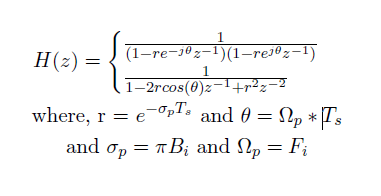
\includegraphics[scale = 0.8]{H.png}
\end{center}
\end{figure}

The Impulse Response of the filter is calculated using the difference equation formula:\\
Summation k=0 to M b[k]y[n - k] = Summation k=0 to N a[k]x[n - k] \\
where, y[n] is the Impulse Response, b[k],a[k] are the numerator and denominator coefficients of H(z) and x[n] is the input Impulse signal\\

Implementing both of these into codes we get the following results.



\subsection{Code}
The code files are included in the .ipynb file included in the submission.

\subsection{Plots}

\begin{figure}[H]
\begin{center}
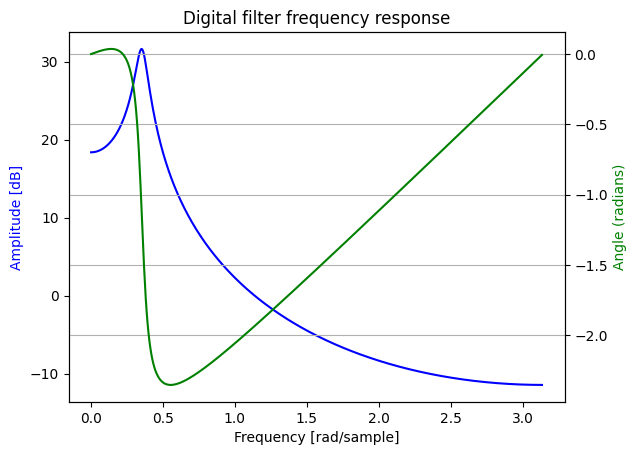
\includegraphics[scale = 0.5]{Q1.png}
\end{center}
\end{figure}


\begin{figure}[H]
\begin{center}
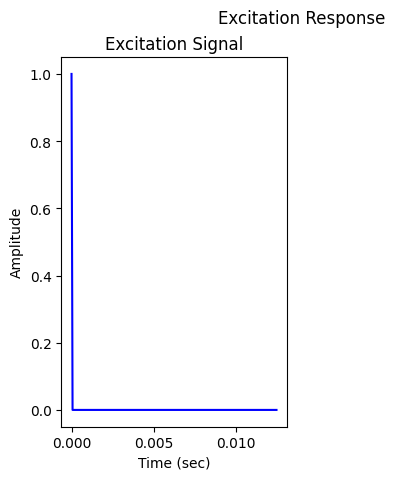
\includegraphics[scale = 0.5]{Q1_Signal.png}
\end{center}
\end{figure}


\begin{figure}[H]
\begin{center}
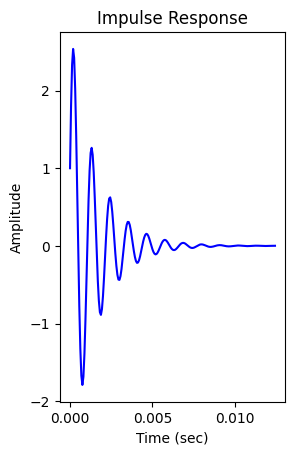
\includegraphics[scale = 0.5]{Q1_Impulse.png}
\end{center}
\end{figure}

\subsection{Observations}

From the plot we can see that the magnitude response is almost maximum at the point Theta = 2*Pie*F1*Ts which matches with our theoretical expectation.

\section{Question 2}

Excite the above resonator (“filter”) with a periodic source excitation of F0 = 160 Hz. You can approximate the source signal by a narrow-triangular pulse train. Compute the output of the source-filter system over the duration of 0.5 second using the difference equation implementation of the LTI system. Plot the time domain waveform over a few pitch periods so that you can observe waveform characteristics. Play out the 0.5 sec duration sound and comment on the sound quality.

\subsection{Solution 2}
The input waveform was approximated using a square-wave having duty-cycle=0.01. \\

Rest the calculation is same as in Question 1.

\subsection{Code}
The code files are included in the .ipynb file included in the submission.

\subsection{Plots}


\begin{figure}[H]
\begin{center}
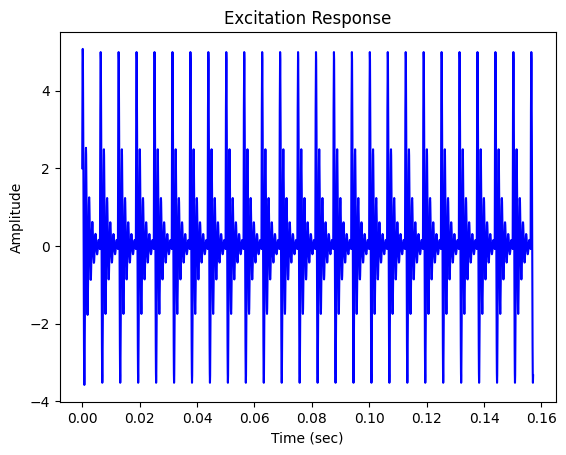
\includegraphics[scale = 0.5]{Q2_Response.png}
\end{center}
\end{figure}


\begin{figure}[H]
\begin{center}
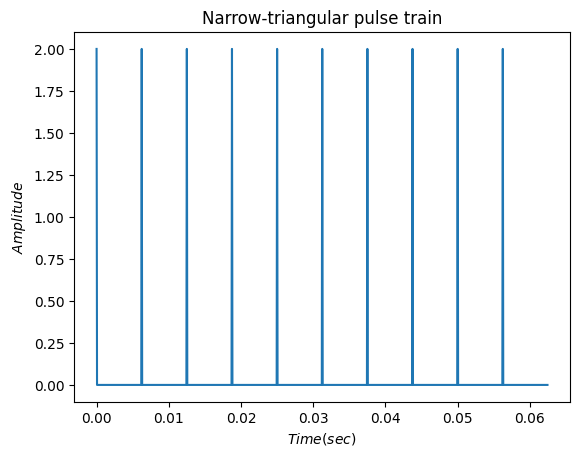
\includegraphics[scale = 0.5]{Q2_Train.png}
\end{center}
\end{figure}



\subsection{Observations}
The sound is very noisy and difficult to predict but seems to resemble vowel a.


\section{Question 3}

Vary the parameters as indicated below; plot and comment on the differences in waveform and in sound quality for the different parameter combinations.\\
(a) F0 = 120 Hz, F1 = 300 Hz, B1 = 120 Hz\\
(b) F0 = 120 Hz, F1=1100 Hz, B1 = 200 Hz\\
(c) F0 = 180 Hz, F1 = 300 Hz, B1 = 120 Hz\\

\subsection{Solution 3}
Same code as the previous 2 parts just convert it to a function and keep changing the variables as given in the question.

\subsection{Code}
The code files are included in the .ipynb file included in the submission.

\subsection{Plots}


\begin{figure}[H]
\begin{center}
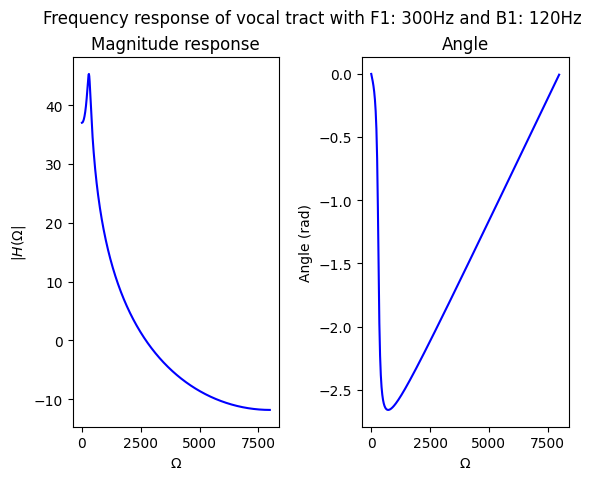
\includegraphics[scale = 0.5]{Q3_A.png}
\end{center}
\end{figure}


\begin{figure}[H]
\begin{center}
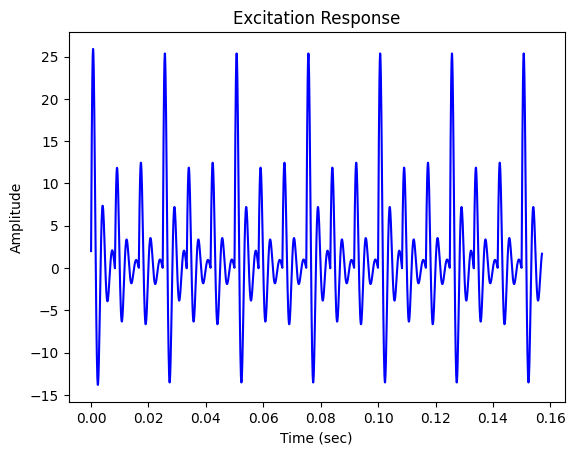
\includegraphics[scale = 0.5]{Q3_AR.png}
\end{center}
\end{figure}



\begin{figure}[H]
\begin{center}
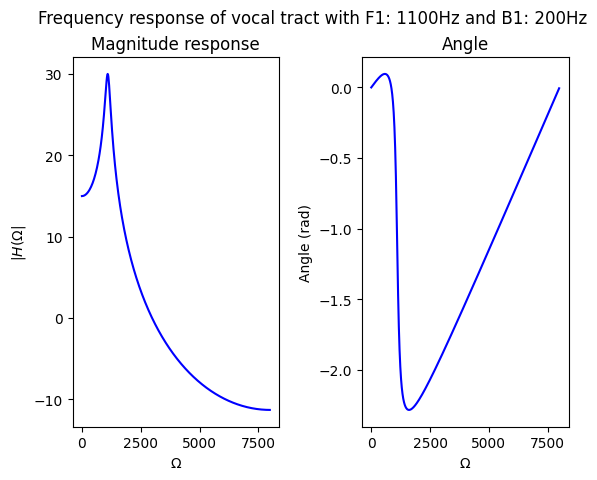
\includegraphics[scale = 0.5]{Q3_B.png}
\end{center}
\end{figure}


\begin{figure}[H]
\begin{center}
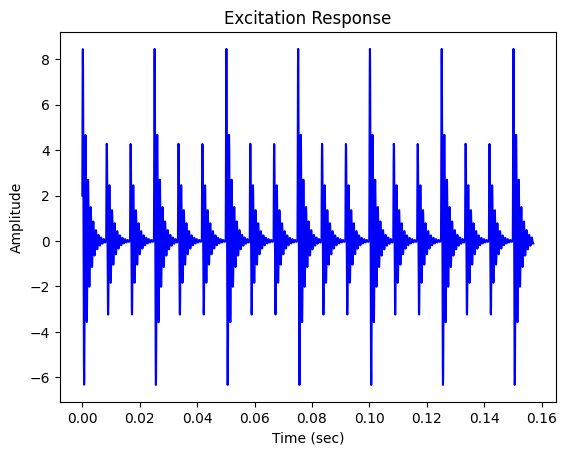
\includegraphics[scale = 0.5]{Q3_BR.png}
\end{center}
\end{figure}


\begin{figure}[H]
\begin{center}
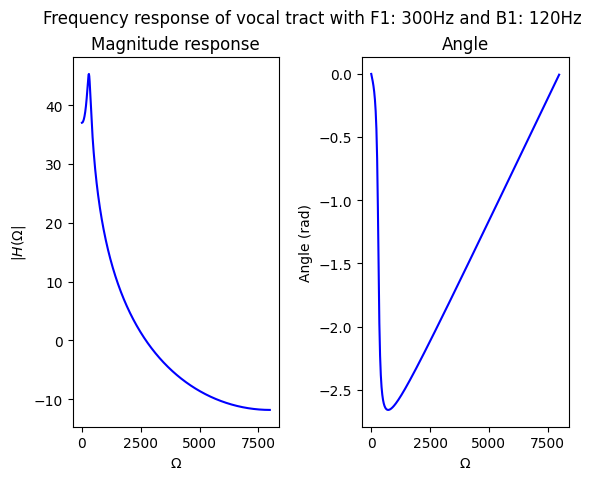
\includegraphics[scale = 0.5]{Q3_C.png}
\end{center}
\end{figure}


\begin{figure}[H]
\begin{center}
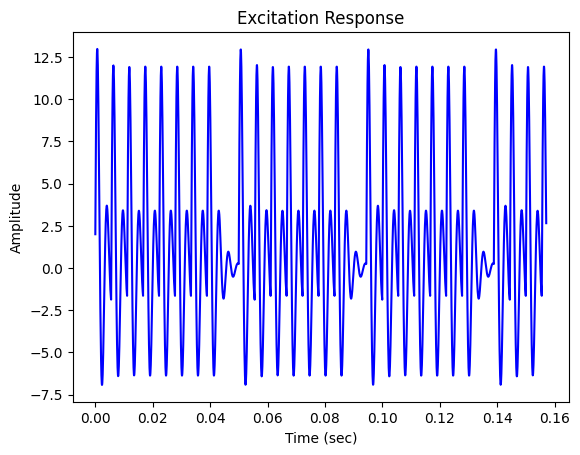
\includegraphics[scale = 0.5]{Q3_CR.png}
\end{center}
\end{figure}

\subsection{Observations}
Although the formant frequencies (and consequently the filter, i.e. the vocal tract characteristics) remain the same in the scenario where the excitation signal frequency (F0) changes from 120 Hz to 180 Hz, the pitch is higher in the scenario where F0 = 180 Hz because the source excitation—the glottal vibration—controls the perceived pitch.\\

The vocal tract's features alter when the formant frequency shifts. Thus, even if the frequency of the excitation signal (glottal vibration) is the same, the output waveform seems to be slightly different, with the second waveform's pitch predominating over the first one.In contrast to the second waveform, which has steep dips to the pulse locally, the first waveform has a significantly smoother time response. \\

Only one peak in each graph of magnitude response because we are seeing only 1 formant.

\section{Question 4}

In place of the simple single-resonance signal, synthesize the following more realistic vowel sounds at two distinct pitches (F0 = 120 Hz, F0 = 220 Hz). Keep the bandwidths constant at 100 Hz for all formants. Duration of sound: 0.5 sec. Comment on the sound quality across the different sounds. Plot a few periods of any 2 examples.\\
Vowel F1, F2, F3\\
/a/ 730, 1090, 2440 \\
/i/ 270, 2290, 3010 \\
/u/ 300, 870, 2240 \\

\subsection{Solution 4}
Again the code and method remains same just change the parameters and observe. This time instead of changing the Signal frequency we change the formant frequency for each corresponding signal frequency.


\subsection{Code}
The code files are included in the .ipynb file included in the submission.

\subsection{Plots}


\begin{figure}[H]
\begin{center}
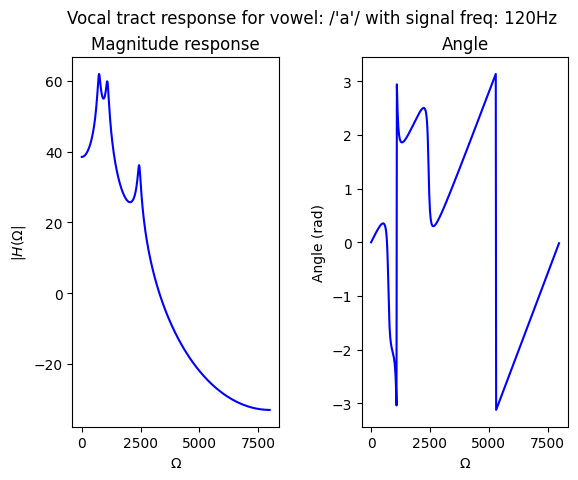
\includegraphics[scale = 0.5]{Q4_A1.png}
\end{center}
\end{figure}


\begin{figure}[H]
\begin{center}
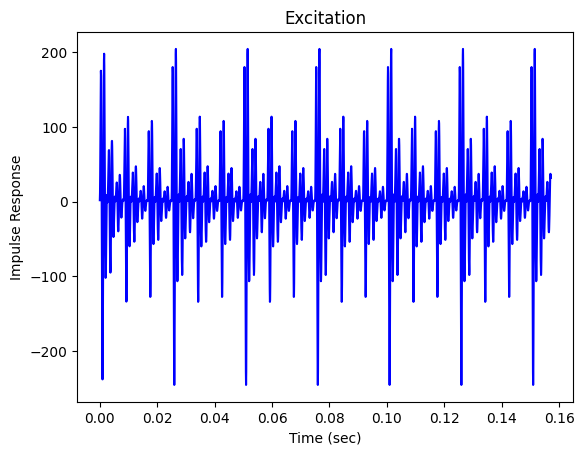
\includegraphics[scale = 0.5]{Q4_A1R.png}
\end{center}
\end{figure}


\begin{figure}[H]
\begin{center}
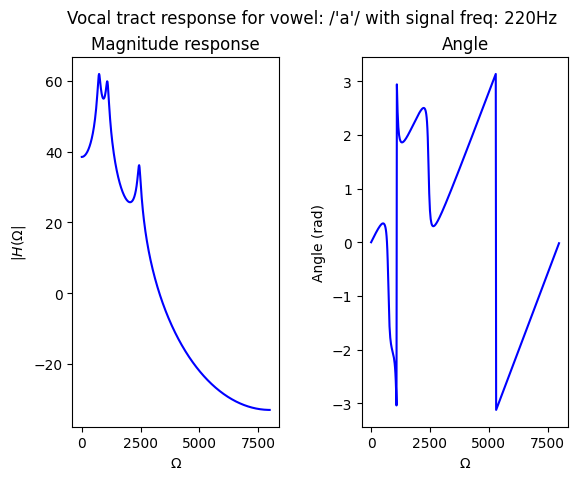
\includegraphics[scale = 0.5]{Q4_A2.png}
\end{center}
\end{figure}


\begin{figure}[H]
\begin{center}
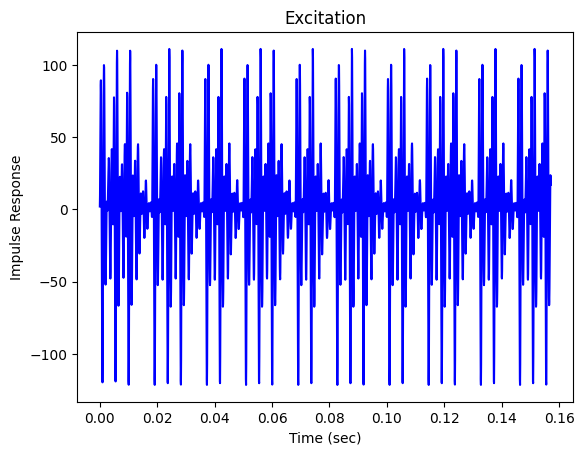
\includegraphics[scale = 0.5]{Q4_A2R.png}
\end{center}
\end{figure}


\begin{figure}[H]
\begin{center}
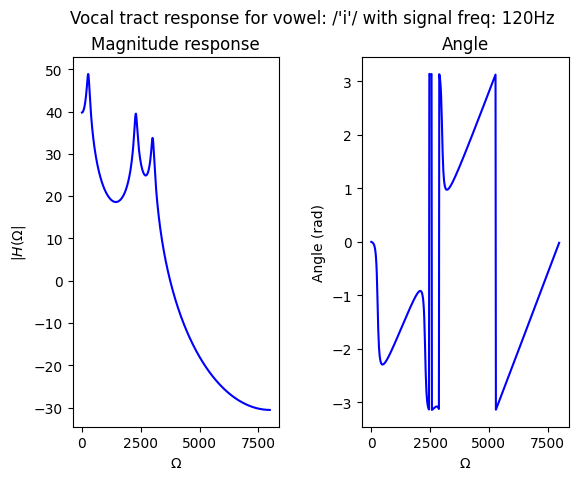
\includegraphics[scale = 0.5]{Q4_B1.png}
\end{center}
\end{figure}


\begin{figure}[H]
\begin{center}
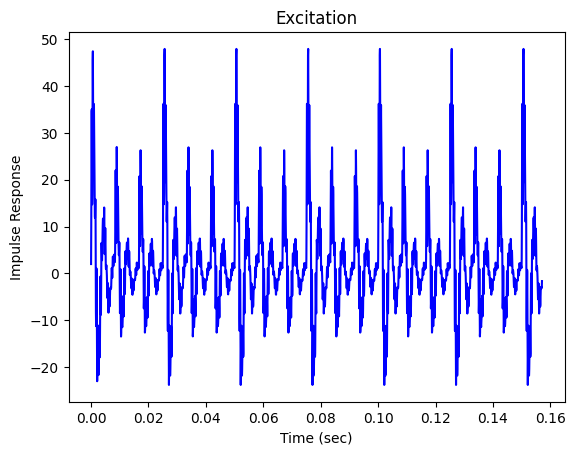
\includegraphics[scale = 0.5]{Q4_B1R.png}
\end{center}
\end{figure}


\begin{figure}[H]
\begin{center}
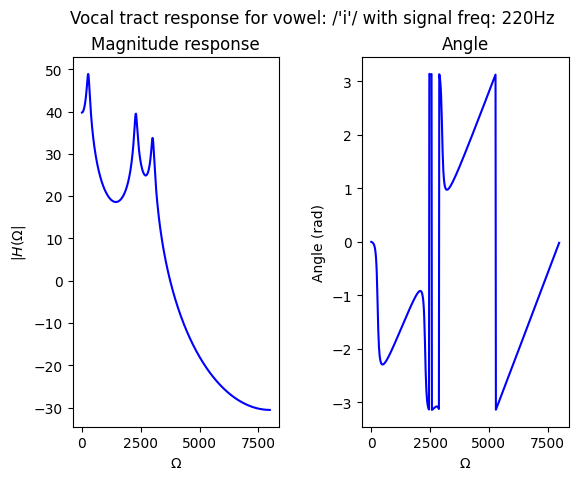
\includegraphics[scale = 0.5]{Q4_B2.png}
\end{center}
\end{figure}


\begin{figure}[H]
\begin{center}
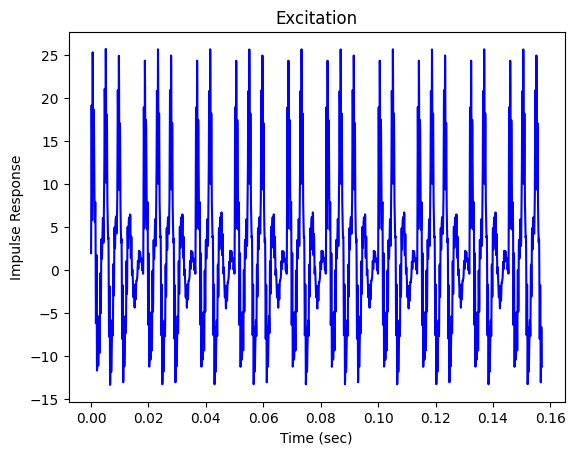
\includegraphics[scale = 0.5]{Q4_B2R.png}
\end{center}
\end{figure}


\begin{figure}[H]
\begin{center}
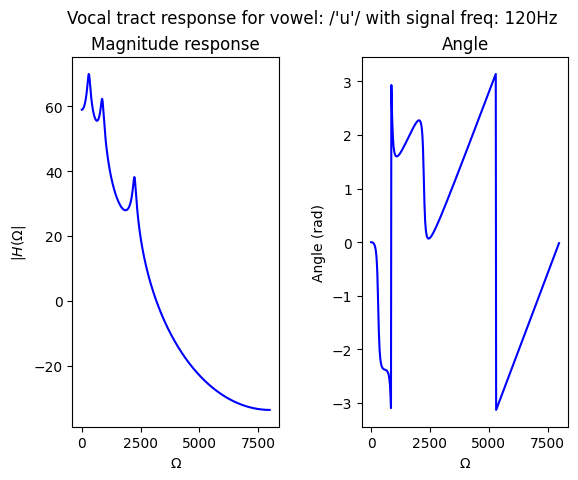
\includegraphics[scale = 0.5]{Q4_C1.png}
\end{center}
\end{figure}


\begin{figure}[H]
\begin{center}
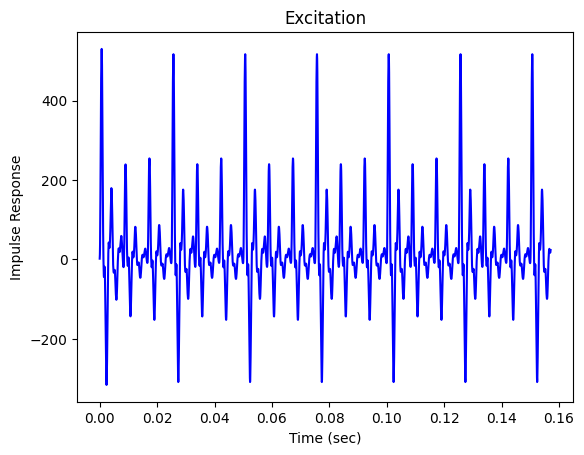
\includegraphics[scale = 0.5]{Q4_C1R.png}
\end{center}
\end{figure}


\begin{figure}[H]
\begin{center}
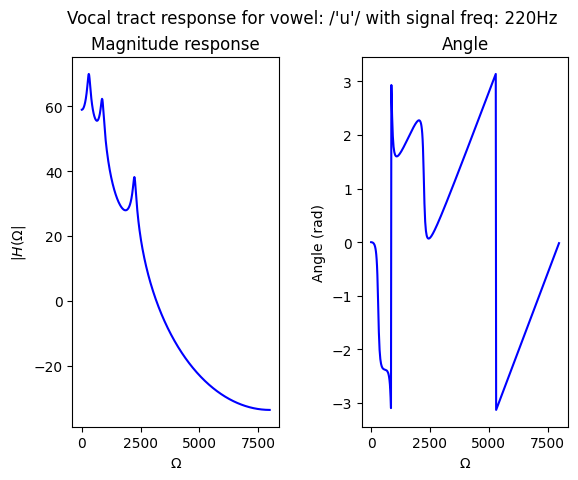
\includegraphics[scale = 0.5]{Q4_C2.png}
\end{center}
\end{figure}


\begin{figure}[H]
\begin{center}
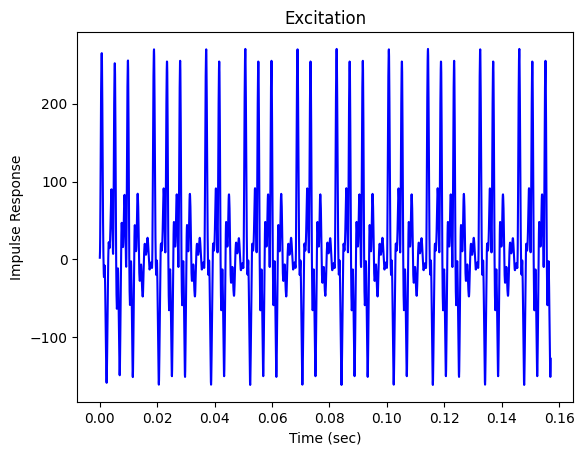
\includegraphics[scale = 0.5]{Q4_C2R.png}
\end{center}
\end{figure}

\subsection{Observations}
Although the vowels can be heard clearly, the noise level remains high. When the F0 frequencies for the various vowels are changed from 120Hz to 220Hz, the pitch of the sounds changes. According to theory, the voice producing the same vowel at F0 = 120Hz should sound like a male voice, whereas the voice producing the same vowel at F0 = 220Hz should sound like a female voice. Upon thorough examination, the wav les do indeed convey this (to a certain extent, albeit with a rather mechanical voice).\\

We can clearly see the formant frequencies in the magnitude response as they corresponds to the 3 peaks in each plot.
    

\end{document}